\section*{1.1 Zero-player game}
Let $G = \langle V, E \rangle$ be a legal graph and $R \subseteq E$ any set of
edges in $G$. We shall define a sequence of moves in a zero-player game
starting from configuration $\mathcal{G}_0 = \mathcal{G},
R_0 = R$ recursively:
\begin{figure}[H]
      \centering
      $R_{k+1} = \{(x,a) \in (E \setminus \bigcup_{i=0}^k R_i):
      a \in fire_{\mathcal{G}_k}(\bigcup_{i=0}^k R_i)\}$\\
      $E_{k+1} = (E_k \setminus R_{k+1}) \cup R_{k+1}^{op}$\\
      $\mathcal{G}_{k+1} = \langle V, E_{k+1} \rangle$
\end{figure}
where $(x, y) \in R_{k+1}^{op} \Leftrightarrow (y, x) \in R_{k+1}$ and weights
are unchanged.

Consider the following problem: given a legal graph
$\mathcal{G} = \langle V, E \rangle$, a set of edges $R \subseteq E$ and an
edge $e \in E$, does there exist a sequence of moves that reverses $e$?\\
\textbf{1. Show that the above problem is P-complete.}\\
1. \underline{$\in \text{P}$}\\
The game can be simulated in a polynomial time. It's easy to see that each timestep (i.e. computing of $R_k, E_k, G_k$
for some $k$) can be done in polynomial time directly from the definition. The game ends after
at most $|E|$ steps (since each edge can occur only in one set $R_i$, we know this directly from
how $R_{k+1}$ is defined). Thus the whole simulation can be performed in polynomial amount of time.\\
2. \underline{P-hard}\\
Circuit value problem (CVP) can be reduced to zero-player flow game.
In CVP, we are given a boolean circuit and its input and we are asked to compute the value of its top node.
A boolean circuit consists of inputs, $\lor$ nodes and $\land$ nodes (there are no
negations, since all negations can be moved to the inputs layer using de Morgan's laws).
A $\lor$ node or $\land$ node has a positive in-degree and its value is either alternative ($\lor$)
or conjunction ($\land$) of its inputs.\\
Let's denote the provided boolean circuit as a directed acyclic graph $C = \langle V_C, E_C, r \rangle$,
where $V_C$ is the set of vertices, $E_C$ the set of directed edges and $r: V \rightarrow \{0,1,\lor,\land\}$
is a funcion mapping a node to its type. If $r(v) \in \{0,1\}$ then $deg_{in}(v) = 0$ (it's an input node).
The only node with $deg_{out} = 0$ is the one for which we want to compute the value.\\
The constructed one-player flow game is $\mathcal{G} = \langle G = (V, E, w), R, e \rangle$, where:
\begin{itemize}
      \item $V = \{v_u :\ u \in V_C, r(u) \in \{0, 1, \lor\}\} \cup
                 \{v_{u_{in}}, v_{u_{out}}\ :\ u \in V_C, r(u) = \land \} \cup \{v_{top}\}$
                 (we copy the input and $\lor$ nodes, split $\land$ nodes into two and add a dummy \textit{top} node)
      \item $E = \{ (v_{a}, v_{b})\ :\ (b, a) \in E_C \} \cup
                  \{(v_{u_{out}}, v_{u_{in}})\ :\ u \in V_C, r(u) = \land \} \cup
                  \{ (v_{top}, v_{u})\ :\ u \in V_C, deg_{out}(v) = 0 \}$
                  (we reverse the edges from the circuit, add an edge from the queried node to \textit{top} and
                  reverse it, for each $\land$ node we add an edge $(\land_{out}, \land_{in})$)
      \item $w(a \in V) = \begin{cases}
                  0\ \ \ \ \ \ \ \ \ \text{ if } a = v_{top}\\
                  0\ \ \ \ \ \ \ \ \ \text{ if } a = v_{u}, r(u) \in \{0,1\}\\
                  deg_{in}(u)\ \ \ \ \text{ if } a = v_{u_{in}} \text{ for some } u \in V_C\\
                  1\ \ \ \ \ \ \ \ \ \text{ otherwise }\\
            \end{cases}$\\
            $w((a,b) \in E) = \begin{cases}
                  deg_{in}(u)\ \ \ \ \text{ if } a = v_{u_{out}}, b = v_{u_{in}} \text{ for some } u \in V_C\\
                  1\ \ \ \ \ \ \ \ \ \text{otherwise}
            \end{cases}$            
      \item $R = \{ v_u\ :\ u \in V_C, r(u) \in \{1\} \}$, those inputs which are set to true
      \item $e = (v_{top}, v_{out})$, where $out$ is the node to evaluate in CVP
\end{itemize}
Below is an example transformation of CVP to zero-player flow game.
\begin{figure}[H]
      \centering
      \caption{An example transformation of CVP to zero-player flow game}
      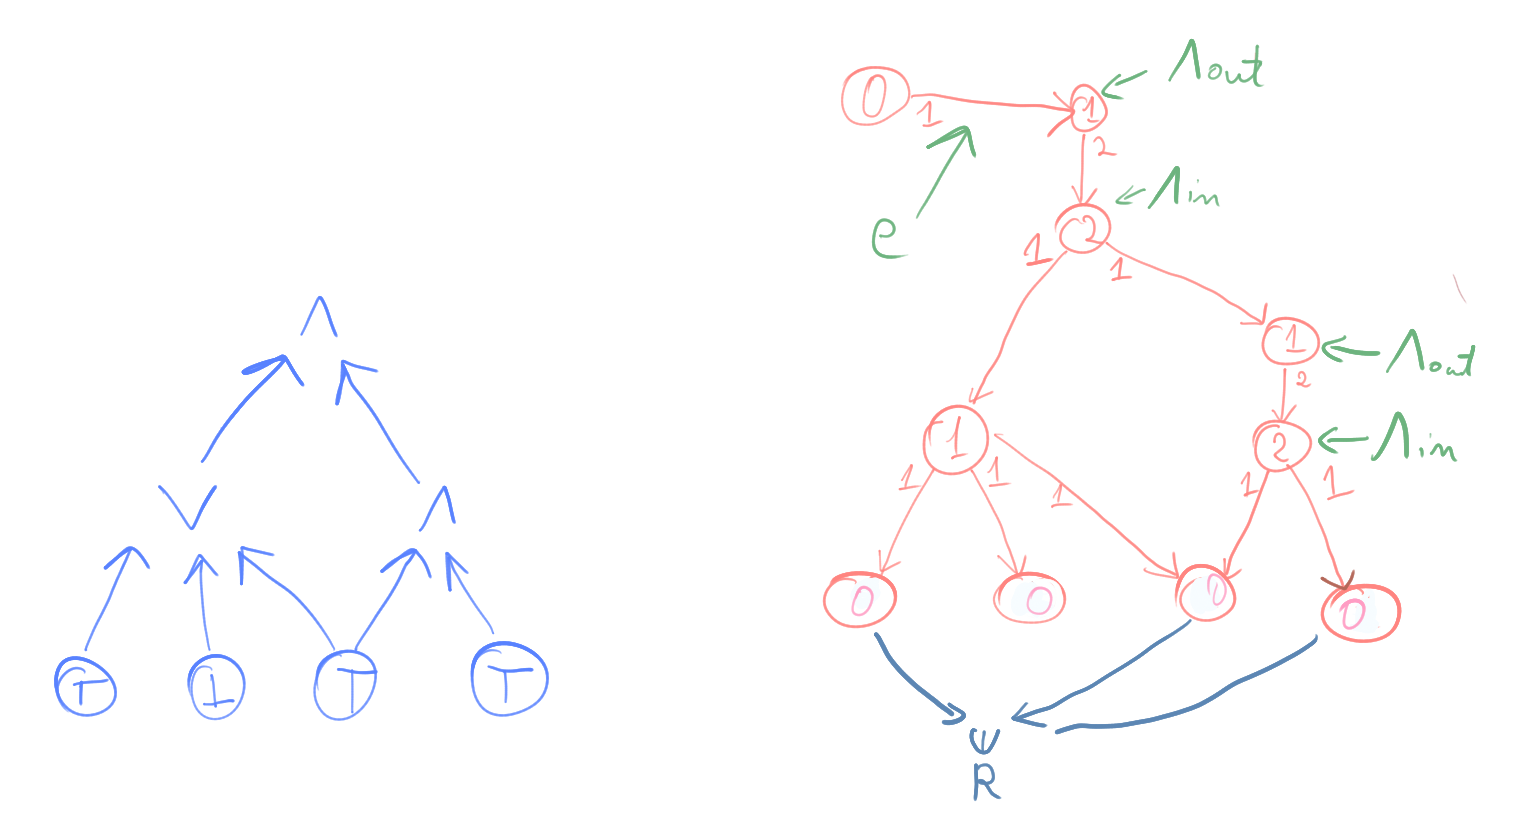
\includegraphics[scale=0.2]{content/graphics/game15.png}
\end{figure}
Note that the edges coming to nodes set to false will never be reversed. True values will propagate
"upwards" the graph.
$e$ will be reversed after some sequence of moves if and only if the circuit evaluates to true.\\

\noindent
\textbf{2. Show that it remains P-complete on planar graphs.}\\
Of course it remains in P on planar graphs, so it suffices to show that it is still P-hard.
Consider my solution from the first subproblem -- I will show how to modify the constructed
graph to make it planar.\\
As advised, I will use the crossover gadget. Consider the figure below, depicting the gadget.\\
\textbf{Observation 1}: The gadget, with the edges directed as shown on the figure is a valid subgraph
(all vertices are firing).\\
\textbf{Observation 2}: The blue edge denoted $B$ can be reversed if and only if $A$ is reversed.
Similarily, the blue edge $D$ can be reversed if and only if $C$ is reversed. Moreover, this will
happen "automatically" (i.e. according to the rules of the zero-player games) -- if $A \in R_k$ for
some $k$, then $B \in R_{k+4}$. If $C \in R_k$ for some $k$, then $C \in R_{k+6}$.
\begin{figure}[H]
      \centering
      \caption{Crossover gadget with initial edges configuration. All nodes have weight 2,
      blue edges have weight 2, red edges have weight 1.}
      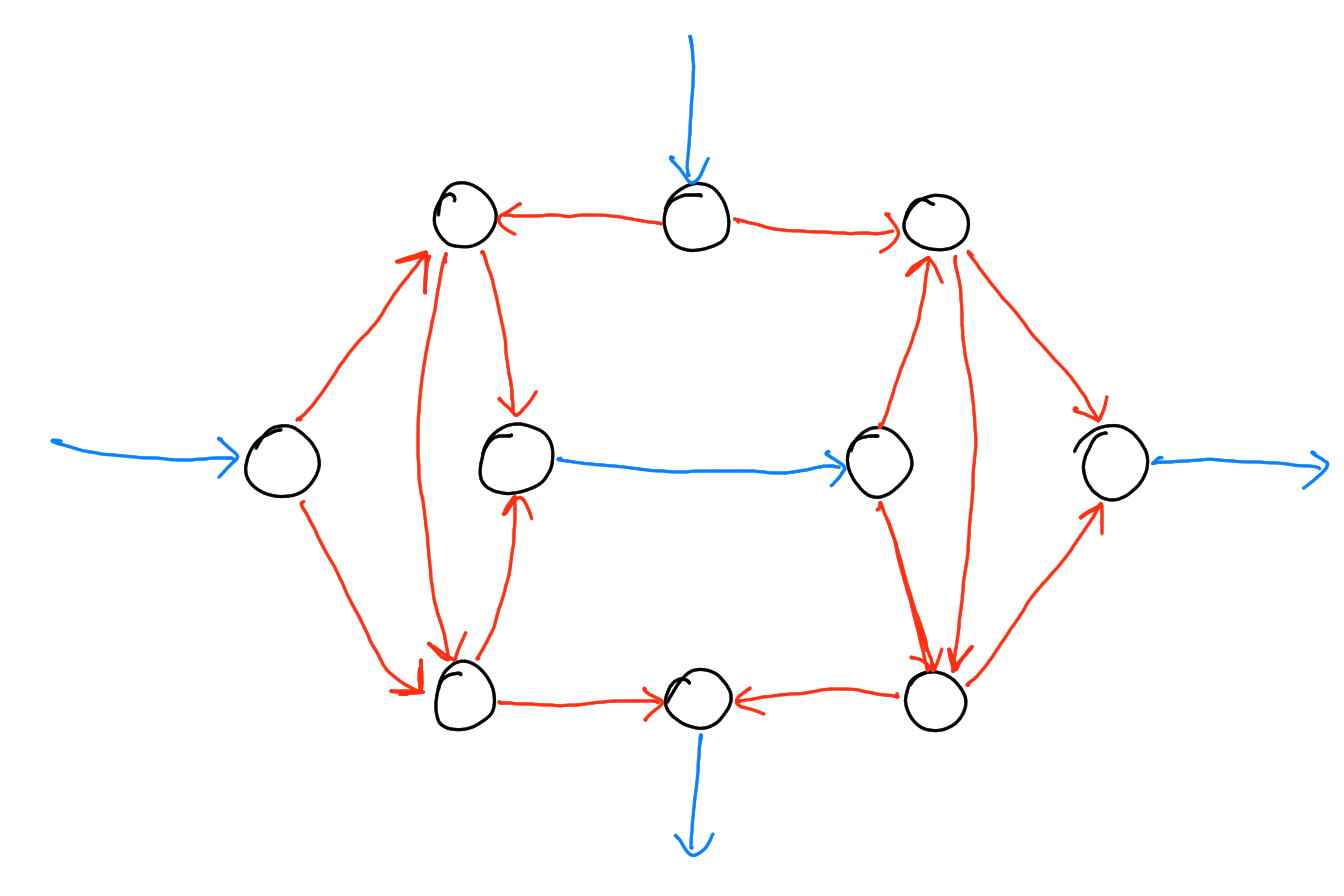
\includegraphics[scale=0.2]{content/graphics/game18.png}
\end{figure}
\noindent
In order to effectively use this widget, I will put one more constraint on the input boolean circuit:
all nodes are placed within "layers" and there are no connections skipping layers. This can be easily
achieved by introducing dummy $\lor$ or $\land$ nodes with one input. See the figure below for an
example of such transformation:
\begin{figure}[H]
      \centering
      \caption{Example transformation of the boolean circuit to get rid of skip-layer connections.}
      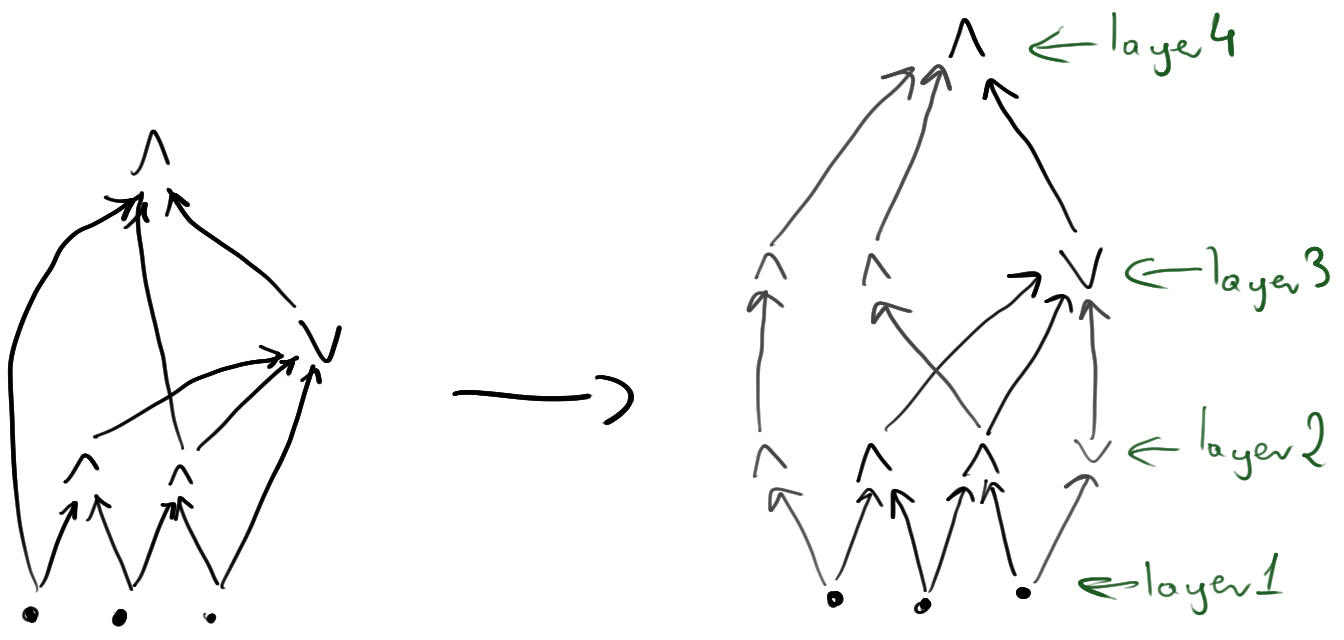
\includegraphics[scale=0.2]{content/graphics/game19.png}
\end{figure}
\noindent
Now, having ensured that two nodes can be connected only if they are on two consecutive layers, 
we need to remove crossing edges.\\
First, we multiply all weights in the graph (both for edges and vertices) by $2$.\\
Then let's take any drawing of the graph on 2D plane such that:
\begin{itemize}
      \item no three edges go through a single point (at most two edges may be intersecting at one point)
      \item two edges may intersect only if they have their ends in the same layers in graph
\end{itemize}
Then in every point, where two edges are intersecting, we place the crossover gadget. Let's assume
we can draw the crossover gadget arbitrarily small, so that it does not introduce intersections with
other edges. From Observation 2 it follows that if there was a sequence of moves winning for in
original graph, then there also exists a (potentially longer) sequence of moves winning for in the
graph with crossover gadgets, and vice versa.
\begin{figure}[H]
      \centering
      \caption{Example transformation of a graph created from a boolean circuit using the method
      from subproblem 1 to a planar graph. The purple dots each denote a crossover gadget.}
      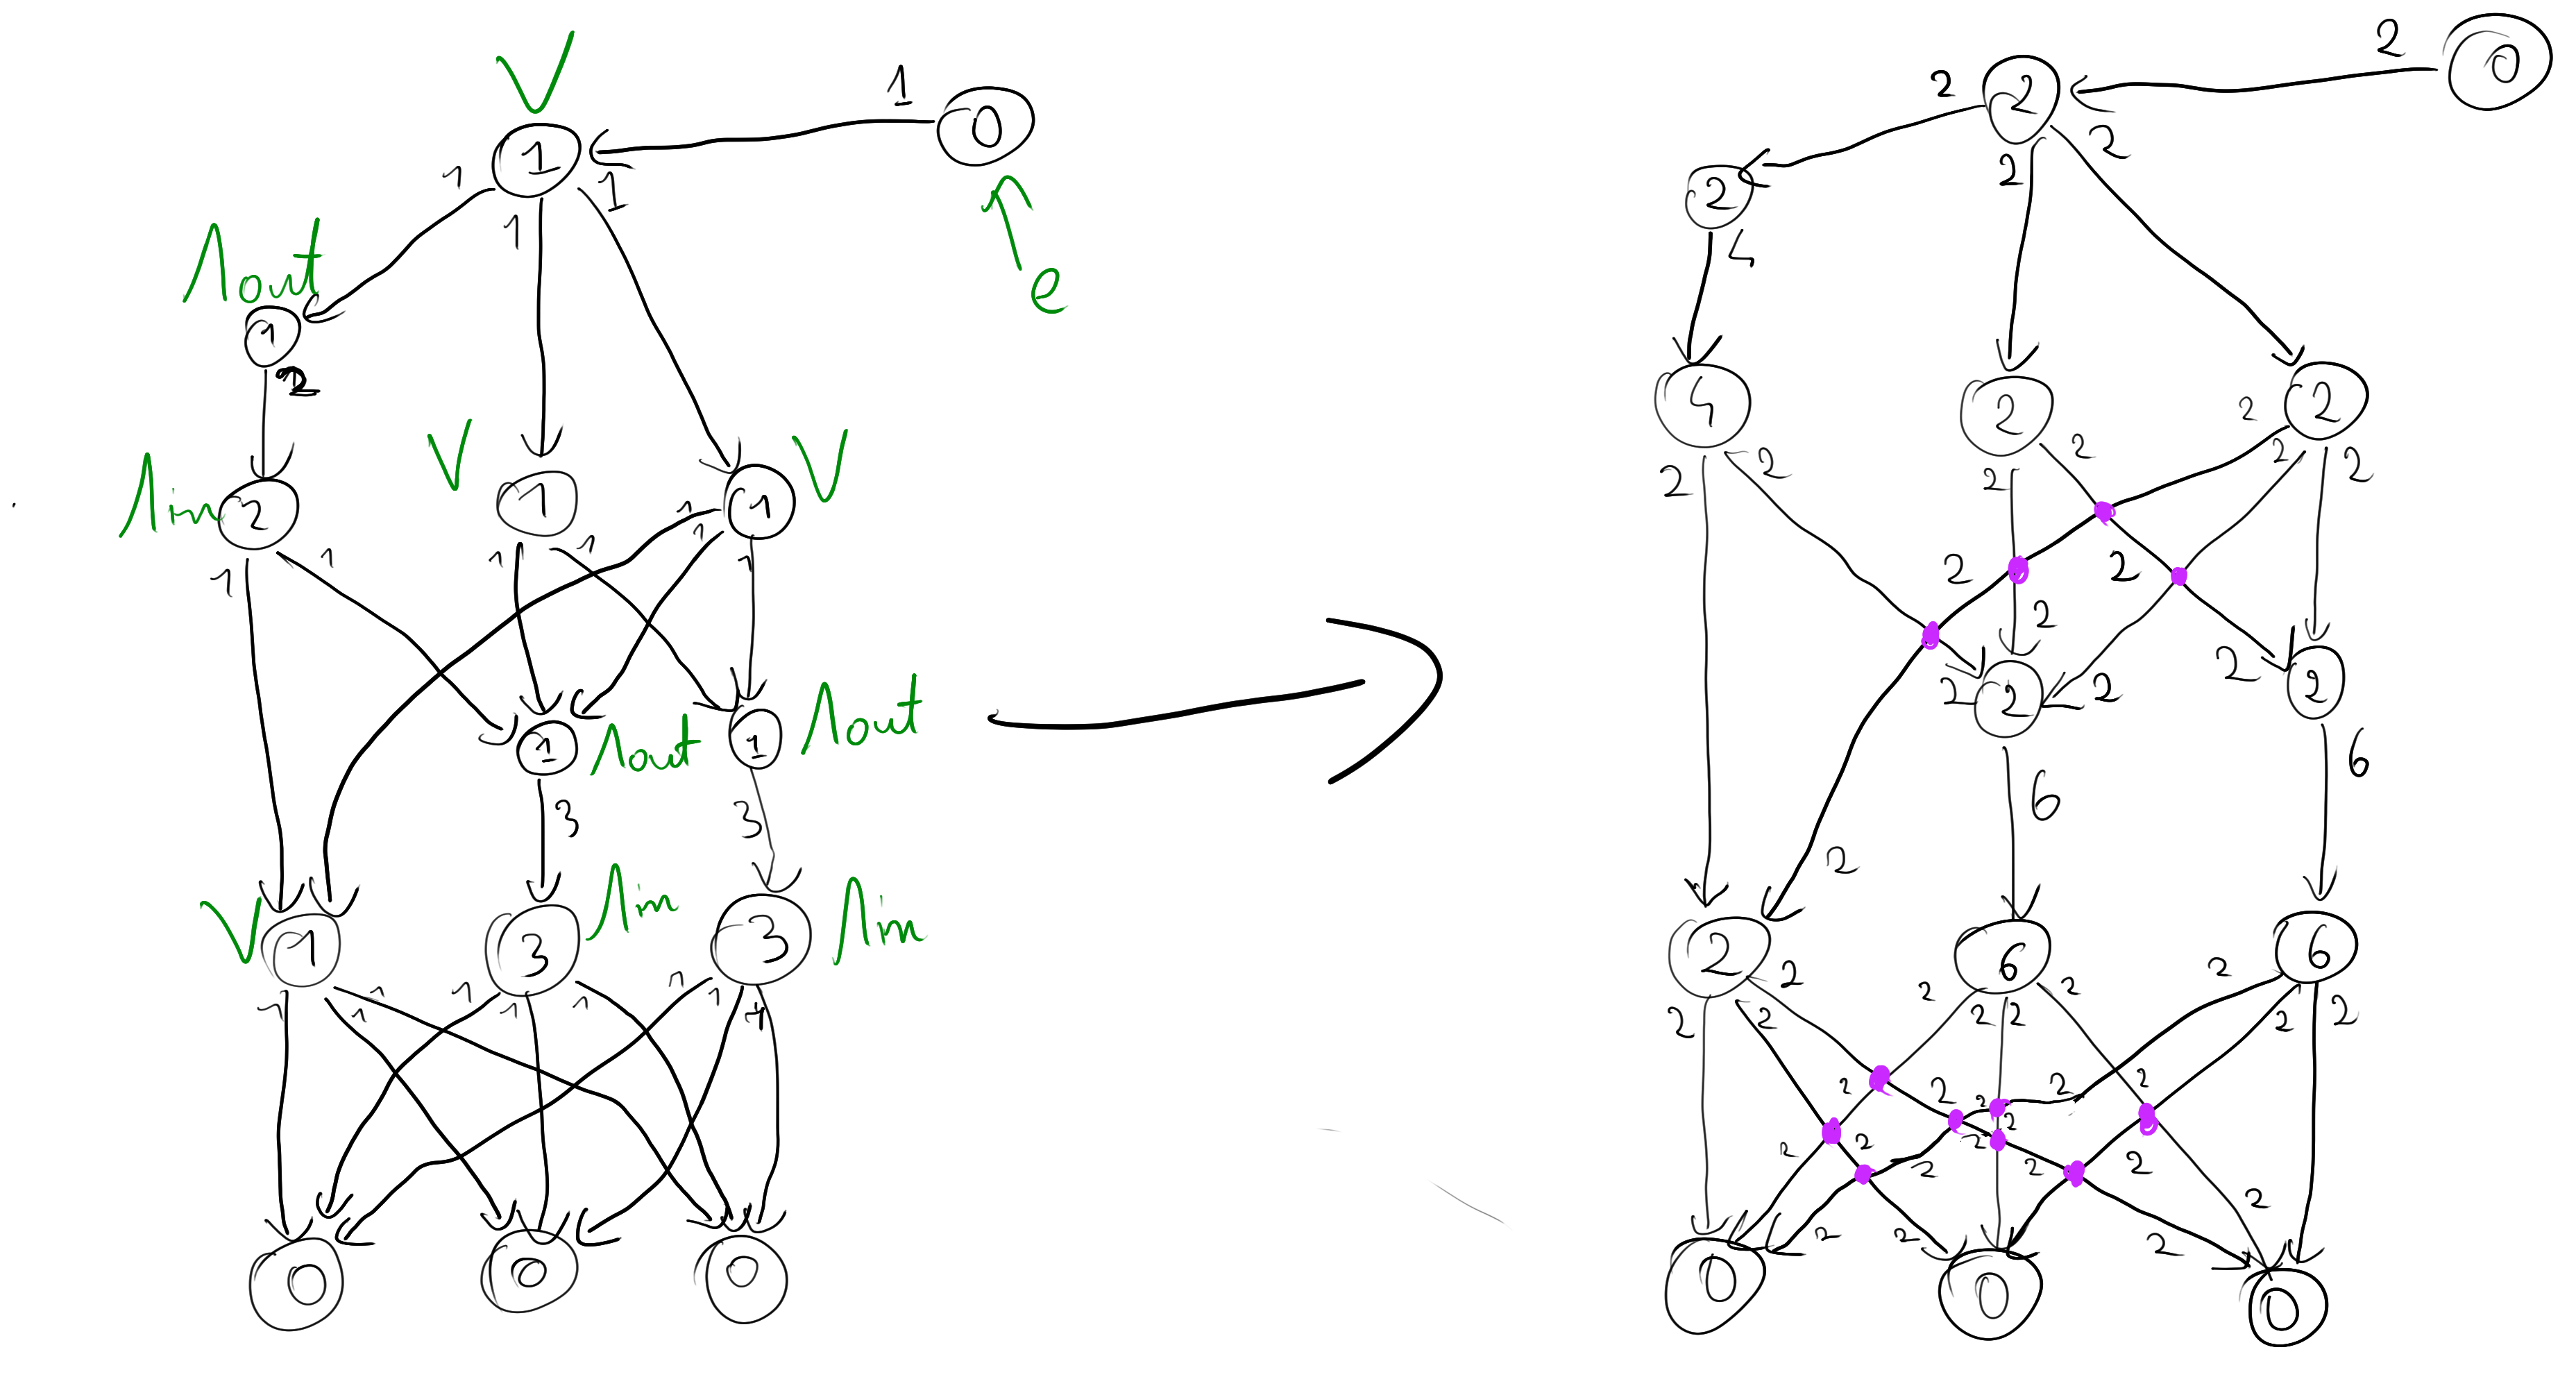
\includegraphics[scale=0.1]{content/graphics/game20.png}
\end{figure}

\noindent
\textbf{
      3. Show that it remains P-complete if we restict to graphs whose vertices have
      degrees at most 3 and the possible weights of both vertices and edges are
      \{1, 2\}.
}\\
Here I will use the solution from the first subproblem but add one more assumption: that the provided
boolean circuit for CVP has vertices with degrees at most $3$, and both input degrees and output degrees
are at most 2 for each node.
It is clear that, with such assumption, my reduction to zero-player flow game from the first subproblem
will produce nodes and edges with weights not larger than $2$. The nodes with weight $0$ (input nodes
and the dummy top node) can be handled easily: input nodes' weights can be changed to $1$ without rendering
the graph illegal. For the dummy top node, it is enough to "plug" it to a small cycle with weights $1$.
See the illustration below:
\begin{figure}[H]
      \centering
      \caption{A small modification of the reduction from the first subproblem to get rid of weights equal to $0$.}
      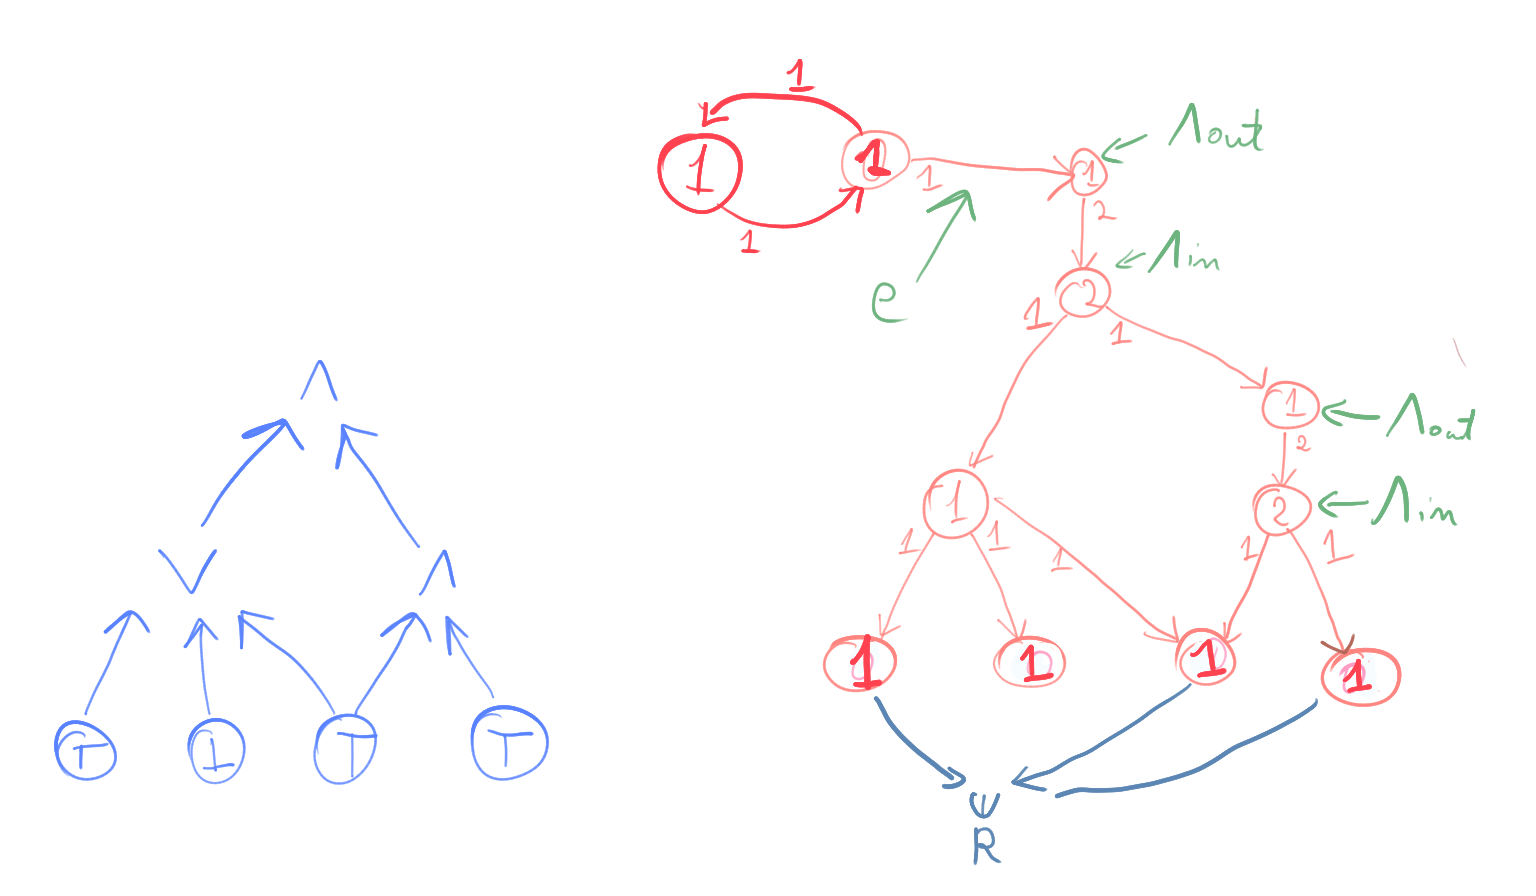
\includegraphics[scale=0.2]{content/graphics/game16.png}
\end{figure}
I have made an assumption that all vertices in the provided circuit have a degree at most 3, and neither input degree
nor output degree is larger than 2 for any node and I will justify that every circuit can be transformed to satisfy this
assumption in reasonable (polynomial) time.

First, every node such that both input and output degree are larger than 1, is split into two, connected by a single edge.
One node handles all input edges, the second -- all output edges. Both nodes perform the same boolean operation as the original
one. This procedure is performed while there is at least one vertex with input and output degree larger than 1.\\
Next, every node with input degree higher than 2 is split into 3 nodes, such that all input edges are divided evenly ($\pm 1$)
between two of them and the third one aggregates their results (refer to the drawing below). This procedure is performed iteratively
while possible.\\
The last step is to perform analogous procedure for outgoing edges. It is also performed iteratively while possible.
\begin{figure}[H]
      \centering
      \caption{
            The three rules to apply iteratively (while possible) to reduce the input and output degrees of
            the nodes in given boolean circuit. For $\lor$ those rules are of course analogous.
      }
      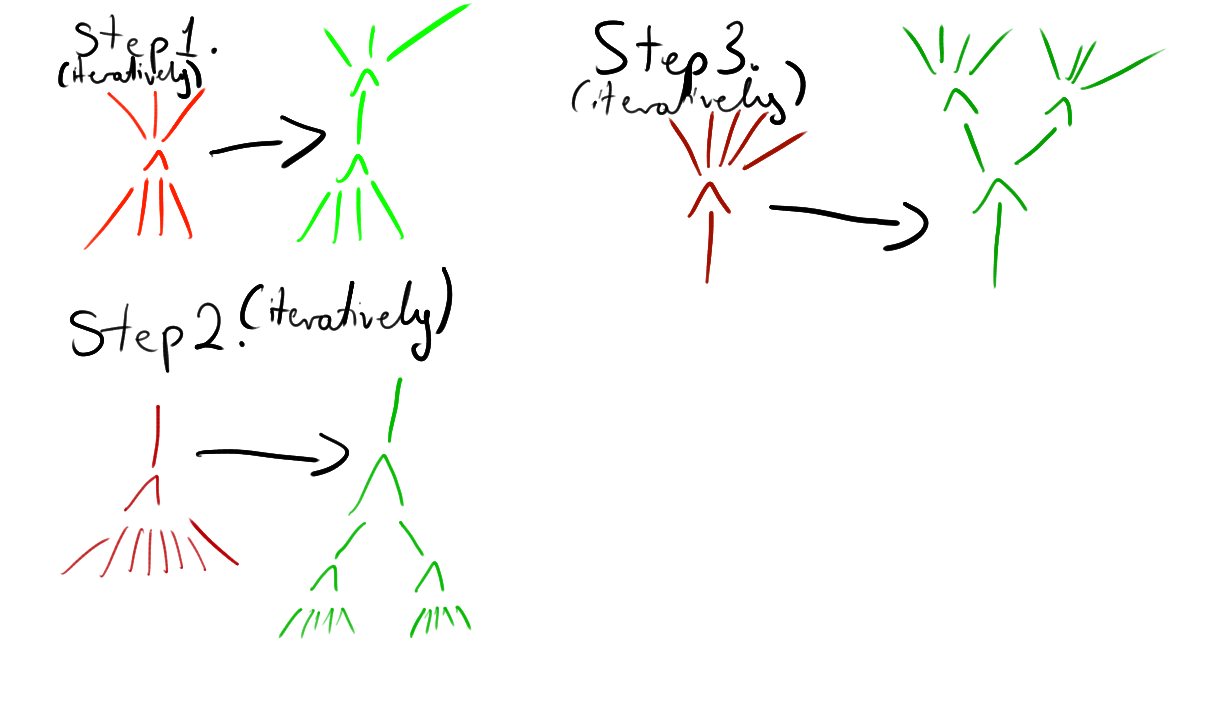
\includegraphics[scale=0.2]{content/graphics/game17.png}
\end{figure}


\subsection*{Unbounded problem}
Consider the following unbounded problem: given a legal graph $G = \langle V, E \rangle$,
a set of edges $R \subseteq E$ and an edge $e \in E$, does there exist a sequence of moves
that reverses $e$?\\
\textbf{1. Show that the unbounded problem is PSpace-complete.}\\
1. \underline{$\in \textsc{PSpace}$}\\
There can be no more than $2^{|E|} \cdot 2^{|E|} \cdot 2^{|E|}$ different combinations of current state of the game:
\begin{itemize}
      \item each edge can either be reversed or not
      \item each edge can either be in $R_k$ or not, for current step number $k$ 
      \item each edge can either be in $R_{k-1}$ or not, for current step number $k$ 
\end{itemize}
The exact value of $k$ is irrelevant to the computation of sets $E_{k+1}, R_{k+1}$. Note that
the above is an upper bound, perhaps a smaller number of different states can be proven.
An example algorithm working in polynomial space is one that just simulates the zero-player unbonded game for
at most $2^{|E| \cdot 3}$ steps, keeping a counter of steps in binary format ($3c \dot |E|$ bits are needed, for some constant $c$).
If edge $e$ has not been reversed during this number of steps, it never will (since some state of the game
has reoccurred and the play will forever loop).\\

\noindent
2. \underline{\textsc{PSpace}-hard}\\
I will show a reduction of QBF problem to the unbounded zero-player game. In fact, I will reuse my
solution from one-player game.\\
Once again, the input to QBF problem is a formula in prenex normal form, where universal and existential quantifiers
alternate, no $\rightarrow$ symbol occurs (implication can be rewritten as an alternative with negation)
and all negations are applied directly to the variables (which can be ensured using de Morgan's laws).
For simplicity, let us also assume that the formula starts with a universal quantifier.
Such assumptions do not reduce the expressive power of possible input formulas.

\noindent
The provided QBF can be decomposed into a tree where every node contains a formula created in a compositional
way from its children.\\
Thus every subformula is of one of the following forms:
\begin{itemize}
      \item $x$ -- a single free variable
      \item $\lnot x$ -- a negation of single free variable
      \item $\theta \lor \delta$, where $\theta$ and $\delta$ are subformulas with no quantifiers, no $\rightarrow$ symbols,
            such that every negation is applied directly to a variable
      \item $\theta \land \delta$, with the assumptions about $\theta$ and $\delta$ as above
      \item $\exists_{x} \psi$, where $\psi$ is a formula, possibly with quantifiers and a potentially non-empty set of
            free variables
      \item $\forall_{x} \psi$, where $\psi$ is a formula, possibly with quantifiers and a potentially non-empty set of
            free variables
\end{itemize}
I will show how to, for each of the above kinds of subformulas, construct a subgraph. The algorithm
is compositional, i.e. does not require any knowledge about nested subformulas. The created subgraphs conform
to two assumptions:
\begin{itemize}
      \item The stray edges (see figure below) are used to provide free variables.
      \item The \textit{output} node fires after some sequence of moves if the formula is satisfied.
\end{itemize}

\noindent
\begin{figure}[H]
      \centering
      \caption{$x, \lnot x$}
      \begin {tikzpicture}[scale=0.7]
            \node[label=$1$,style={draw=black,circle}] (A) at(0,0) {$x$};
            \path[->] (A) edge node[above] {1} +(-2,0);
      \end{tikzpicture}\\
      \begin {tikzpicture}[scale=0.7]
            \node[label=$1$,style={draw=black,circle}] (A) at(0,0) {$\lnot x$};
            \path[->] (A) edge node[above] {1} +(-2,0);
      \end{tikzpicture}
\end{figure}

\noindent
\begin{figure}[H]
      \centering
      \caption{$\phi \land \psi$}
      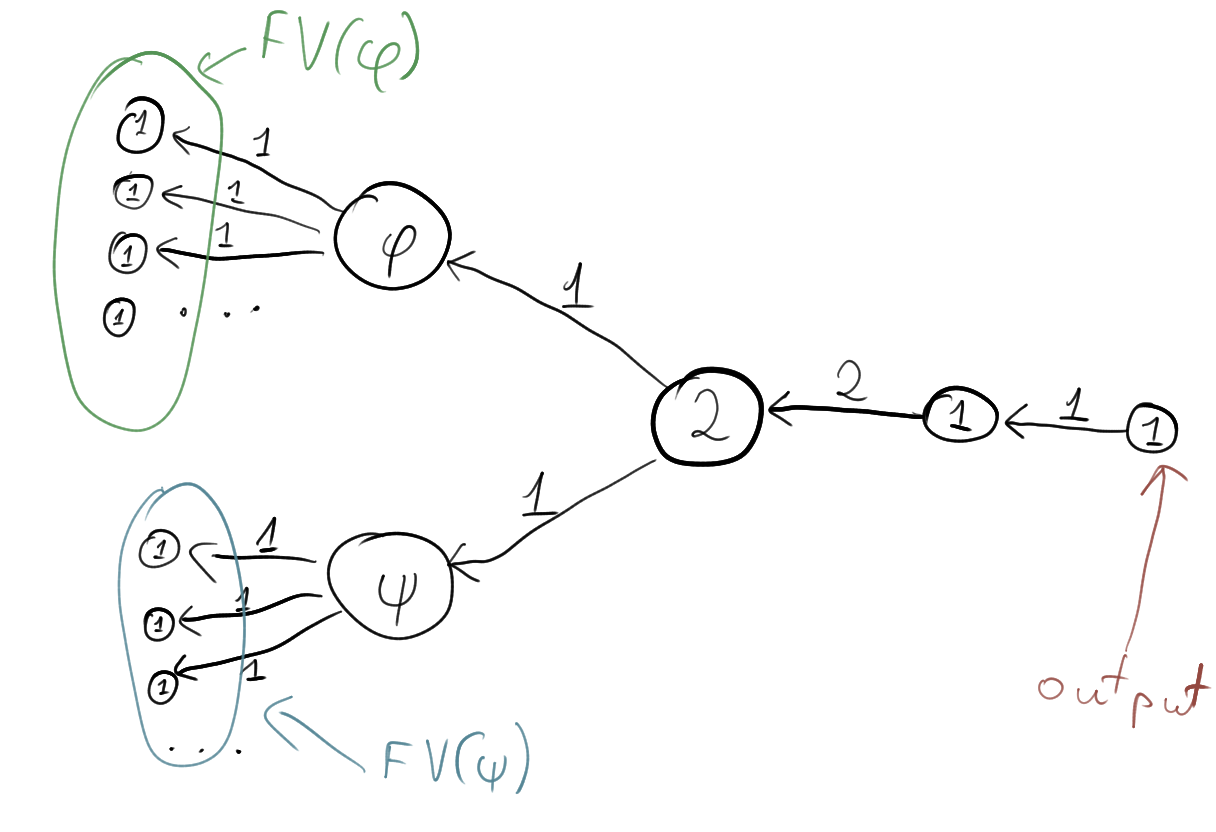
\includegraphics[scale=0.15]{content/graphics/game10.png}
\end{figure}

\noindent
\begin{figure}[H]
      \centering
      \caption{$\phi \lor \psi$}
      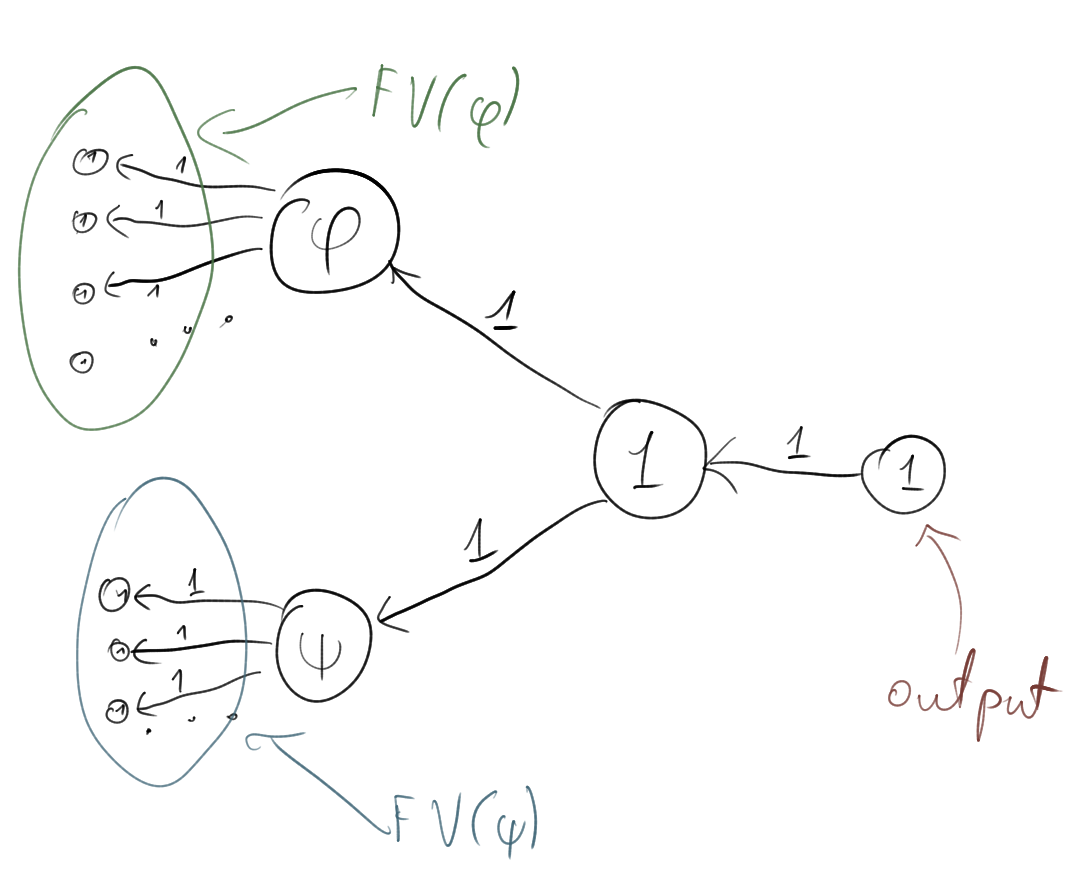
\includegraphics[scale=0.15]{content/graphics/game11.png}
\end{figure}

\noindent
\begin{figure}[H]
      \centering
      \caption{$\forall_{x} \phi$}
      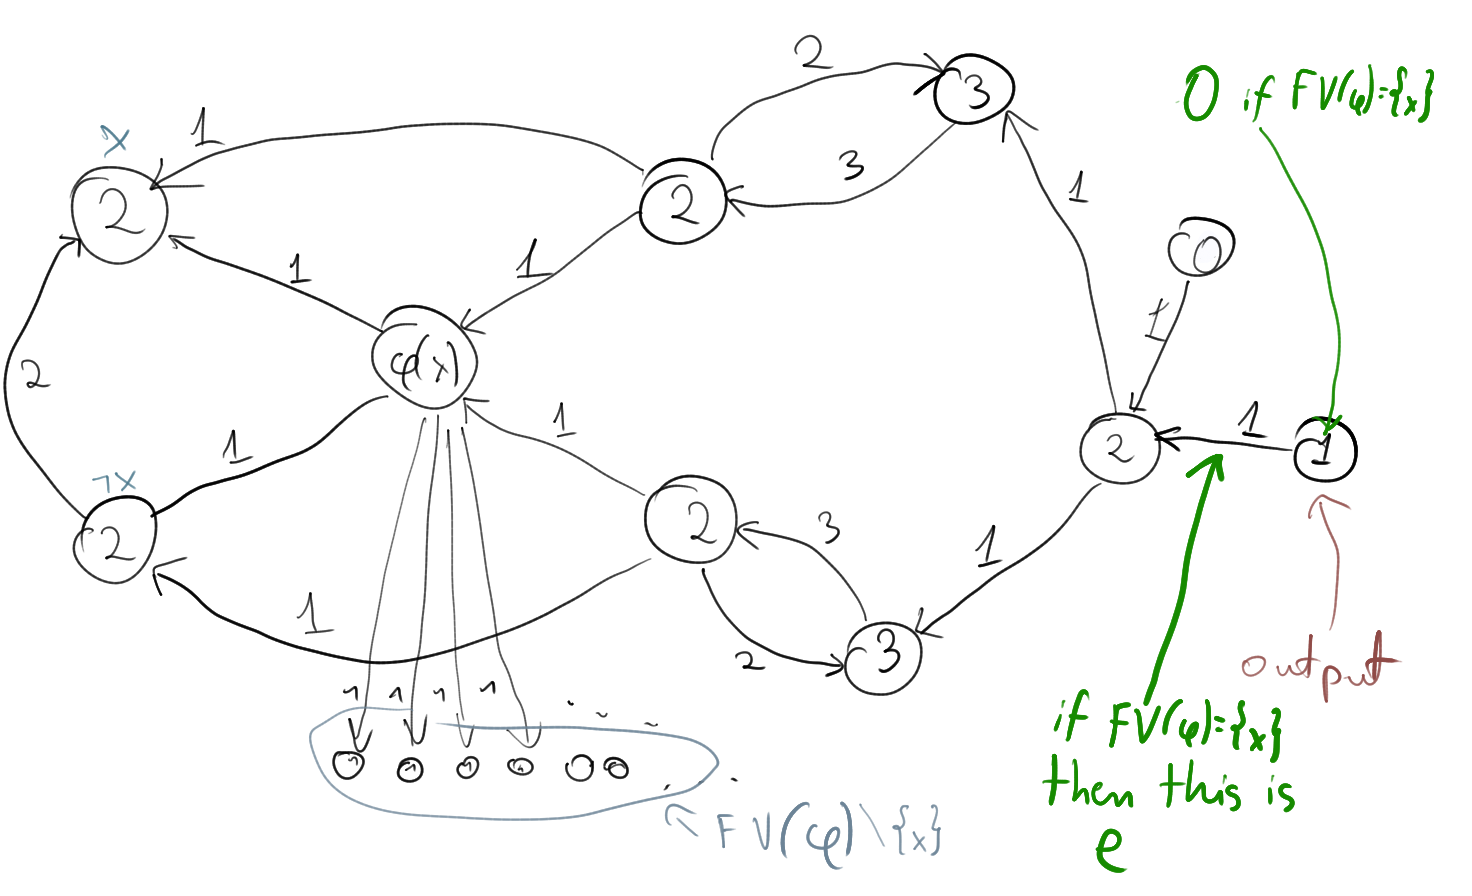
\includegraphics[scale=0.15]{content/graphics/game12.png}
\end{figure}

\noindent
\begin{figure}[H]
      \centering
      \caption{$\exists_{x} \phi$}
      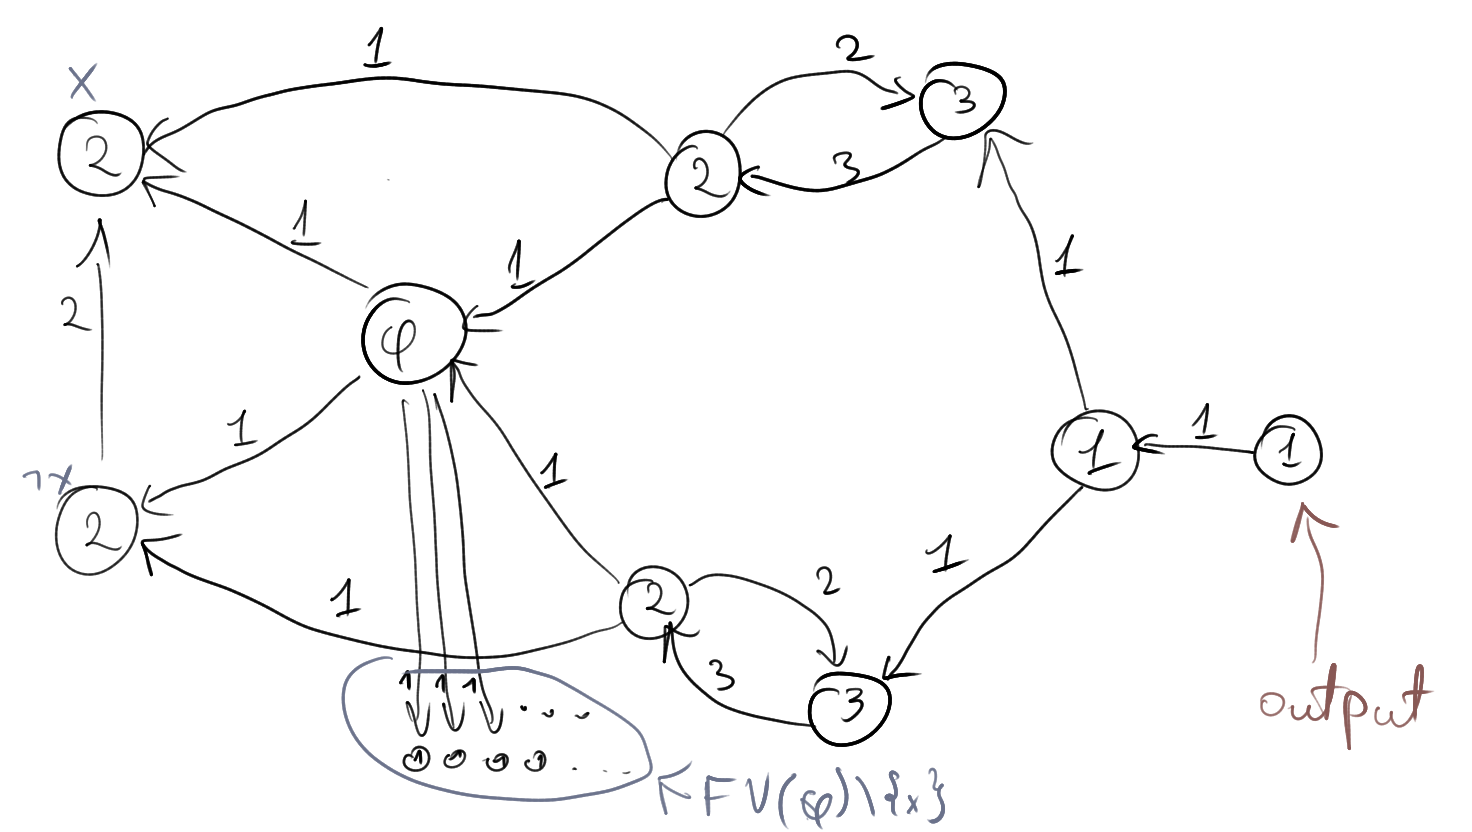
\includegraphics[scale=0.15]{content/graphics/game13.png}
\end{figure}

\noindent
Following the above constructions, we create an unbounded flow game $\langle G, R, e \rangle$
from the input QBF formula, where:
\begin{itemize}
      \item $G$ is the constructed graph
      \item $e$ is the output edge from the root subformula ($\forall_{x1}...$) graph
      \item $R$ is a singleton consisting of the edge $\langle \lnot x_1, x_1 \rangle$ with weight 2
            in the root subformula ($\forall_{x_1}...$)
\end{itemize}
A small difference between one-player and unbounded zero-player game here is that the graph will not
stay legal at all timesteps. However, it is easy to check that the "errors" will not propagate to the
output nodes in subformulas.\\
In total, the edge $e$ can be reversed in some sequence of moves if and only if the given QBF formula is true.